\section{Ejercicio 2}
\subsection*{Instrucción}
En este apartado se desea implementar la siguiente operación:
\par
\vspace{0.15cm}
\texttt{takeOutOfService(backToService : date):} 
pone un coche que está en servicio fuera de servicio, registra la fecha hasta la que el coche permanecerá fuera de servicio y busca un coche para sustituir al que se pone fuera de servicio. El sustito debe cumplir
una serie de restricciones: 

\begin{itemize}
    \item Debe estar asignado a la misma oficina que el coche sustituido.
    \item Debe ser del mismo modelo.
    \item Finalmente, debe estar en servicio.
\end{itemize}

Además, se menciona la funcionalidad que pone un coche fuera de servicio en servicio. Sin embargo, no se pide su implementación


\subsection{Patrón de Diseño utilizado}

Para poner un coche fuera de servicio hay que considerar varios factores.

Por un lado, el coche que está fuera de servicio no puede ser puesto fuera 
de servicio de nuevo. 

Por otro lado, si un coche está en servicio, pero es sustituto del otro coche, 
tampoco puede ponerse fuera de servicio.

Un coche que está en servicio, puede ser alquilado, mientras que el coche que está fuera de servicio 
o que es el sustituto del otro coche, tampoco puede ser alquilado.

Como se puede apreciar, el comportamiento del coche varía en función de su estado. Por eso, hemos considerado usar el \texttt{Patrón Estados}dado que nos permite definir el comportamient del coche de manera flexible sin cambiar la estructura interna de la clase.

En nuestro caso, un coche puede estar en uno de los dos posibles estados:

\begin{itemize}
    \item \texttt{En servicio:} el coche en este estado está disponible para ser alquilado. 
    \item \texttt{Fuera de servicio:} el coche en este estado está fuera de servicio por varias razones (reparación, ITV, etc.).
    
\end{itemize}



\subsection{Efectos sobre el Diagrama de Diseño}
\begin{figure}[H]
    \centering
     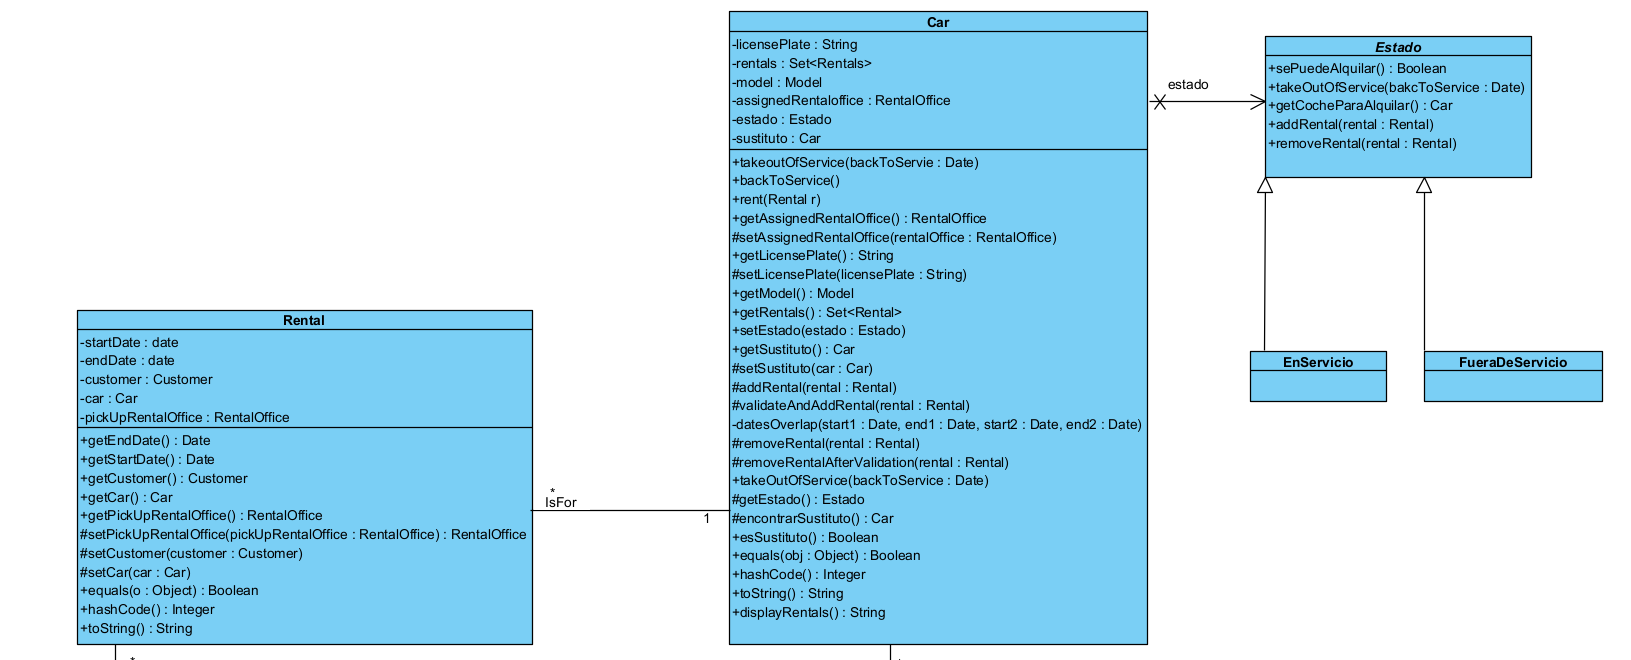
\includegraphics[width=1.0\linewidth]{assets/diagramas/UML_Apartado2.png}
     \caption{Diagrama de Diseño modificado para Ejercicio2}
\end{figure}

Con el fin de implementar el patrón escogido hemos tenido que insertar una clase abstracta \texttt{Estado}
que representa el estado de coche.
Además, hemos tenido que insertar dos clases que heredan de la clase mencionada: 
\begin{itemize}
    \item \texttt{EnServicio:} la instancia de la clase Car con estado de este tipo está en servicio. Este tipo permite poner un
                            coche fuera de servicio y alquilarlo
    \item \texttt{FueraDeServicio:} la instancia de la clase Car con estado de este tipo está fuera de servicio. No permite alquilar un coche, pero permite
                            alquilar el sustituto asociado, si es que existe.
    
\end{itemize}

\subsection*{Métodos adicionales de la calse \texttt{Car}:}
\begin{itemize}
    \item \texttt{protected void validateAndAddRental(Rental rental):} es un método de la calse \texttt{Car} que antes de asignar un alquiler comprueba si 
    no se solapa on ningún otro que ya está asignado al coche. Para realizar esta comprobación se usa un método privado  \texttt{datesOverlap}        
    \item \texttt{protected Car encontrarSustituto():} una vez que el coche se pone fuera de servicio, se usa este método para encontrar sustituto en función de los 
    p usa en la redefinición del método \texttt{takeOutOfService(Date backToService)} en la
    subclase \texttt{EnServicio}, esta parte se trata más adelante. 
    \item \texttt{public boolean esSustituto():} comprueba si el coche actual es sustituto o no. Esta información es necesaria a la hora de 
    asignar un alquiler, dado que si un coche se usa como sustituto no puede ser alquilado como un coche normal.   
    
\end{itemize}
\subsection*{Métodos de la clase \texttt{Estado}:}
\begin{itemize}
    \item \texttt{public abstract boolean sePuedeAlquilar():} indica si se puede alquilar un coche o si no se puede alquilar un coche. Su implementación en la clase \texttt{EnServicio} 
    devuelve \texttt{verdadero}, mientras que la de la clase \texttt{FueraDeServicio} devuelve \texttt{falso}. Cabe destacar su implementación en la clase \texttt{EnServicio}.
    \begin{lstlisting}[style = javaNormal, language=Java]
        public boolean sePuedeAlquilar(){
          return !context.esSustituto();
        }    
    \end{lstlisting}
    Como se puede observar, usamos el método \texttt{esSustituto()}. Esta implementación, la consideramos correcta dado, que la única condición para 
    que un coche en servicio no se pueda alquilar es que sea un sustituto.       
    \item \texttt{public Car getCocheParaAlquilar():} es un método que devuelve la instancia del coche o el sustituto en función 
    del estado del coche. 
    \item \texttt{public boolean esSustituto():} comprueba si el coche actual es sustituto o no. Esta información es necesaria a la hora de 
    asignar un alquiler, dado que si un coche se usa como sustituto no puede ser alquilado como un coche normal.
    \item \texttt{public boolean addRental(Rental rental):} añade alquiler al propio coche si este está en servicio o al sustituto, si está fuera
    de servicio y tiene uno.
    \item \texttt{public boolean removeRental(Rental rental):} sigue la misma lógica que el método \texttt{addRental(Rental rental)}, pero en vez de añadir
    el alquiler, este se elimina.
    
\end{itemize}


\subsection{Implementación de \textit{takeOutOfService : date}}
\begin{lstlisting}[style = javaNormal, language=Java] 

    introducir codigo aqui

\end{lstlisting} % Código en el documento "codigosEj2"

\newpage
